\questionheader{Question 2: Which way is the slowdown moving?}

\noindent
\begin{minipage}[t]{0.56\textwidth}
\vspace{0pt}
\begin{itemize}
    \item \textbf{(a) Symmetric layer:} Only sensors 19, 20 and 21 get nonzero predictions: the neighbour weight $b$ at 19 and 21 and the self weight $a$ at 20, against true values 1, 0 and 0. The squared error is smallest at $a = 0$ and $b = 0.5$ (total 0.5). The layer cannot tell which neighbour the slowdown moves to, so it splits the spike into two half-size copies. Over 20 steps the bump never moves; it stays at sensor 20 and spreads out, its peak falling from 1.0 to 0.41 (Figure 1).
    \item \textbf{(b) Directional layer:} With separate weights for the sensor ahead and behind, copying only the sensor ahead (weights 0, 0, 1) is exact for every snapshot. A 1D convolution with kernel [0, 0, 1] and wrap-around padding does the same on the ring. Separate weights remove the left--right symmetry that trapped the layer in (a).
    \item \textbf{(c) Adding history:} With weights 0 (self), 1 (both neighbours) and $-1$ (own previous value), the layer is exact for both directions. A sensor's previous value equals the neighbour the slowdown has just moved to, so subtracting it leaves only the neighbour it is coming from. The direction comes from time, not from the edges.
\end{itemize}
\end{minipage}
\hfill
\begin{minipage}[t]{0.42\textwidth}
\vspace{2pt}
{\footnotesize\textbf{Figure 1: 20-step rollout, true motion (left) vs the fitted symmetric layer (right)}}\\[2pt]
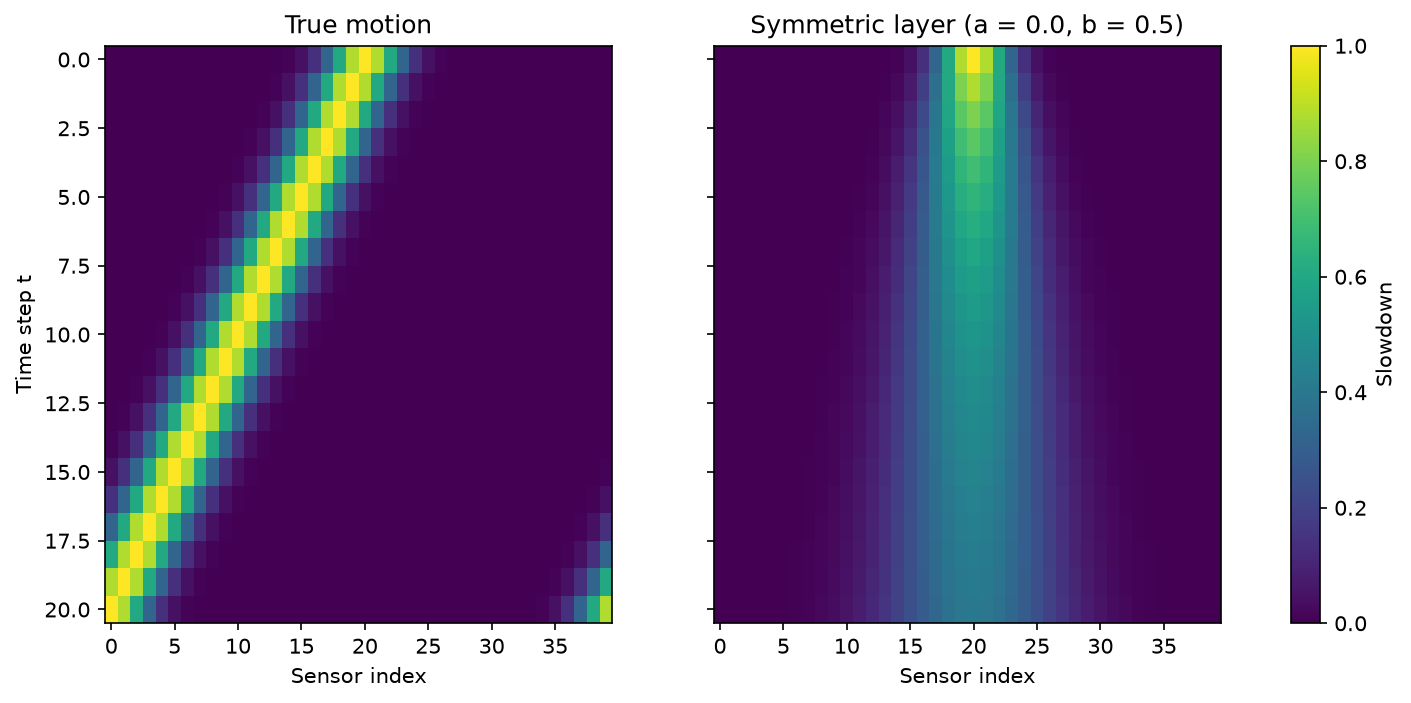
\includegraphics[width=\textwidth]{figures/q2_heatmaps.png}
\end{minipage}
\vspace{4pt}
